
\chapter{MacOS Tips}


\section{Cut, Copy and Paste}
In the text environment:
The cut shortcut is \keyword{Command + x}.
The copy shortcut is \keyword{Command + c}.
The paste shortcut is \keyword{Command + p}.

In the file system:
There is no cut shortcut, but you can get the cut+paste function with \keyword{Command + c} following \keyword{Command + Option + v}.
\keyword{Command + Option + c} functions copyping the file absolution path.



\section{Spotlight}

The shortcut is \keyword{Command + Space}. Spotlight can do all kinds of things, from locating files to answering basic questions to solving math problems.

\begin{figure}[H]
  \centering
  
\includegraphics[width=0.8\textwidth]{spotlight.png}
  \caption{Spotlight}
\end{figure}

\section{Close Apps From App Switcher}

When you're in the \keyword{Command + Tab} view, press the \keyword{Q} key with command held down to close an open app.


\section{Hide a Window}

Just press \keyword{Comand + h} to hide the current window.
The app will disappear into the background, but you can get it back by clicking on the icon on the dock or using Command + Tab.

\section{Hide All Windows}

You can hide all of the windows except for the window for the app you're currently using by pressing \keyword{Option + Command + H}.

\section{Switch Between Subwindows}

\keyword{Command + Number} to switch to the the n-th subwindows.

\section{Delete Files}

\keyword{Command + Delete} to move the files into Trash.
\keyword{Command + Option + Delete} to delete permanently without moving the files into Trash.


\section{Screenshots}

\keyword{Command + Shift + 3} takes a screenshot.
\keyword{Command + Shift + 4} lets you select an area of the screen to screen screenshot.
\keyword{Command + Shift + 5} brings up an interface that lets you select the screenshot or record.

\section{Look for Your Mouse}

If you ever lose your mouse in a sea of windows onscreen, just shake it, and the cursor will automatically enlarge.


\section{Force Quit}

Inevitably your Mac will freeze up and force you to quit some apps.
There's no "Ctrl Alt Delete" here — instead, you hit \keyword{Command + Option + Escape} to shut tasks down the hard way.
This is a bit faster than right-clicking on each troublesome app yourself.


\section{Move Window Background}

You can move windows without bringing them to the foreground by holding Command as you drag it around.


\section{Startup Login Items}

If you ever feel like changing which apps load whenever you boot up your Mac, you can go to System Preferences > Users \& Groups > Login Items, then add, check, and uncheck whatever you want to prioritize.


\begin{figure}[H]
  \centering
  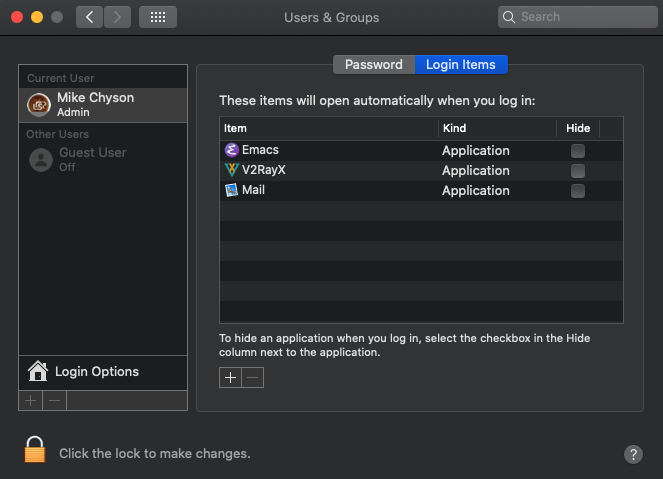
\includegraphics[width=0.8\textwidth]{login-items.png}
  \caption{Login Items}
\end{figure}


\section{Accent Marks}

Whenever you need an accent mark (or related foreign character), just hold down the appropriate letter, and a list of relevant options will pop up.

\section{Rearrange Icons in Menu Bar}

If you do keep the menu bar around, though, you can rearrange the icons within it by holding Command and dragging them around.
You can also use this to remove certain icons off the menu bar completely.


\section{Split View}

If you're only working on a couple of things, you can take them into a cleaner, Split View layout by holding down the rightmost (or green) button at the top of a given window.




\section{Finder Control}
You can switch Finder view with the \keyword{Command + [1-4]}.


\section{Maximize and Unmaximize the Window}

\keyword{Ctrl + Command + f}

\section{What's Your Preference?}

Working in an application and need to access the preferences for that application? Tap \keyword{Command + ,}, and you’re in.

\section{A Really Smart Search}

So, you’ve set your Safari search preferences to something other than Google? (Safari Preferences>Search choose a new search engine in the drop-down menu.)
Now here’s a super-fast way to search using Spotlight:

\begin{itemize}
\item Type \keyword{Command + Space} to open Spotlight
\item Type your query
\item Then type \keyword{Command + b} and you’ll be taken directly to the search results in default search engine.
\end{itemize}


Now you can tap \keyword{Command + Tab} to return to your previous application, where the information you just found may come in useful.


\section{Preview Shortcuts}

\begin{description}
\item[Command + 1] Continuous Scroll
\item[Command + 2] Single Page
\item[Command + 3] Two Pages
\item[Option + Command + 1] Hide Sidebar
\item[Option + Command + 2] Thumbnails
\item[Option + Command + 3] Table of Contents
\item[Option + Command + 4] Highlights and Notes
\item[Option + Command + 5] Bookmarks
\item[Option + Command + 6] Contact Sheet
\item[Command + [] Back
\item[Option + Command + g] Go to Page
\end{description}

\section{Minimize a Window}

\keyword{Command + m}

\section{Close a Window or Tab}

\keyword{Command + w}

\section{New a Tab}

\keyword{Command + t}

\section{Inspector}

\keyword{Command + i}